%  Typ dokumentu - článek, prezentace aj.
\documentclass[english]{article}

%  Nastaví vstupní a výstupní kódování znaků (encoding) a lokalizace
\usepackage[T1]{fontenc}
\usepackage[utf8]{inputenc}
\usepackage[english,czech]{babel}
\usepackage{icomma}
\usepackage{lmodern}

%  Formát papíru a odsazení od jeho okrajů
\usepackage[letterpaper]{geometry}
\geometry{verbose,tmargin=1.5cm,bmargin=2cm,lmargin=2cm,rmargin=2cm}

%  Umožňuje pracovat s grafikou
\usepackage{graphicx}
\usepackage{bigstrut}

%  Automaticky odsadí i první paragraf v každé sekci
\usepackage{indentfirst}

%  Umožňuje rozdělovat obsah na více sloupců
\usepackage{multicol}

%  Umožňuje používat hypertextové odkazy, nastavuje jejich barvu a
%  vlastnosti
\usepackage[unicode]{hyperref}
\hypersetup{
colorlinks=true, citecolor=blue, filecolor=blue, linkcolor=blue,
urlcolor=blue
}

%  Umožnění odstranění italiky u jednotek
\newcommand{\unit}[1]{\mathrm{#1}}

%  Formátování stránek, empty = odstraní číslování
% \pagestyle{empty}

%  Řádkování
\linespread{1.2}

%  Lepší zobrazování matematiky (rozšíření sum o \limits atd.)
\everymath{\displaystyle}

% Umožní psát přes \mathbb{N/R/Q/..} množiny čísel
\usepackage{amssymb}

%  Velikost fontu matematických výrazů v dokumentu lze pro danou
% základního fontu dokumentu upravit pomocí:
% \DeclareMathSizes{X}{Y}{Z}{U} kde:
% X je velikost fontu v dokumentu, pro kterou se matematika upraví
% Y je standartní velikost fontu matematiky
% Z je velikost fontu zmenšených (vnořených výrazů)
% U je velikost fontu ještě více zmenšených (vnořených výrazů).
\DeclareMathSizes{10}{10.5}{9}{9}

%  Nastaví autora, název, datum, skupinu měření apod. (můj vlastní
% příkaz, umožní znovu-použití v dokumentu)
\newcommand{\Author}{David Roesel}
\newcommand{\Coauthor}{Tereza Schönfeldová}
\newcommand{\Institute}{FJFI ČVUT v Praze}
\newcommand{\Subject}{FYZIKÁLNÍ PRAKTIKUM I}
\newcommand{\Group}{7}
\newcommand{\Circle}{ZS 5}
\newcommand{\Title}{Úloha \#12 \\Stirlingův stroj}
\newcommand{\Date}{8.11.2013}

% Začátek dokumentu - Formátování na výstup
\begin{document}

% Interní proměnné, možno zobrazovat u prezentací, používají se při
% generování pomocí \titlepage apod.
\author{\Author}
\title{\Title}
\date{\Date}

%  Lokalizace některých názvů do češtiny
\renewcommand{\figurename}{Obr.}
\renewcommand{\tablename}{Tab.}
\renewcommand{\refname}{Reference}

% --- Hlavička dokumentu -----------------------------------------------

\setlength{\parindent}{0cm}
\begin{multicols}{2}
\textbf{\Subject \\
        \Institute \\[0.1cm]
%\large  \Title \\[0.5cm]
\Title \\[0.5cm]
}
\begin{tabular}{rlrl}
\large Datum měření: & \Date & \large Skupina: & \Group \\
\large Jméno: & \Author & \large Kroužek:  & \Circle\\
\large Spolupracovala: & \Coauthor &\large Klasifikace:\\
\end{tabular}

\begin{flushright}

\includegraphics[scale=0.28]{../../_meta/fjfi_standart.pdf}
\hspace{0.2cm}

\includegraphics[scale=0.28]{../../_meta/cvut_standart.pdf}
\end{flushright}
\end{multicols}
\hrule
\vspace{0.5cm}

% ----------------------------------------------------------------------


% --- Tělo dokumentu ---------------------------------------------------
\setlength{\parindent}{0.5cm}

\section{Pracovní úkoly}
	\begin{enumerate}
	\item DÚ: V domácí přípravě diskutujte rozdíl mezi $pV$ diagramem Carnotova cyklu a Stirlingova procesu. Dále porovnejte účinnosti těchto dvou procesů a diskutujte, který je účinnější.
	\item Spočítejte celkový výkon lihového vařiče $P_{L}$.
	\item Správně ztotožněte osy na osciloskopu (napětí) s osami $pV$ diagramu.
	\item Naměřte a následně nakreslete do grafu závislost elektrického výkonu $P_{e}$ na počtu otáček $N$. Tuto závislost proložte polynomem 2. stupně a určete při jakých otáčkách má stroj největší výkon. Alespoň pro tři body grafu zaznamenejte příslušný $pV$ diagram.
	\item Sestavte Stirlingův stroj jako chladničku, zaznamenejte $pV$ diagram ve chvíli kdy $\triangle T < 0$ a diskutujte jeho tvar.
	\item Porovnejte elektrickou práci $W_{e}$ a plochu pod křivkou $W_{pV}$ v $pV$ diagramu.
	\item Spočítejte účinnosti a diskutujte rozdíly mezi výsledky.
	\end{enumerate}

\section{Vypracování}

\subsection{Použité přístroje}
	Stirlingův motor, lihový vařič se skleněným závětřím, $pV\ NT$ měřící jednotka, 2-kanálový osciloskop, regulovatelný zdroj 0-20 V, líh, kabely, ampérmetr, voltmetr, odporová dekáda, mobilní telefon.

\subsection{Teoretický úvod}

\subsubsection{Stirlingův stroj}
	Celý pokus probíhá měření s teplovzdušným Stirlingovým motorem. Tento motor prochází při každém cyklu postupně čtyřmi fázemi:
	\begin{enumerate}
	\item Izotermální expanze, systému je dodáváno teplo a koná se na něm práce
	\begin{center} $V_{1} \rightarrow V_{2},\qquad p_{1} \rightarrow p_{2},\qquad T_{1}=\mathrm{konst}.$ \end{center}
	\item Izochorický proces, dochází k ochlazování plynu
	\begin{center} $T_{1} \rightarrow T_{2},\qquad p_{2} \rightarrow p_{3},\qquad V_{2}=\mathrm{konst}.$ \end{center}
	\item Izotermální komprese, systém vydává teplo a koná práci
	\begin{center} $V_{2} \rightarrow V_{1},\qquad p_{3} \rightarrow p_{4},\qquad T_{2}=\mathrm{konst}.$ \end{center}
	\item Izochorický proces, dochází k ohřívání plynu
	\begin{center} $T_{2} \rightarrow T_{1},\qquad p_{4} \rightarrow p_{1},\qquad V_{1}=\mathrm{konst}.$ \end{center}
	\end{enumerate} 
	
	Stirlingův motor obsahuje dva písty s posunutou fází, přičemž ve vodorovné části nedochází ani ke změnám objemu - pohyb pístu v ní pouze mění teplotu. Všechny změny objemu koná vertikální píst.
	
	Dodáváme-li do izolovaného systému teplo, platí
	\begin{equation}
	dQ = dU +dW,
	\end{equation}
	kde $dQ$ je změna tepla v systému, $dU$ je změna jeho vnitřní energie a $dW$ je vykonaná práce.
	
	Stirlingův motor teplo uvolněné jako odpad zachytává a recykluje. Tento tzv. princip regenerace zvyšuje účinnost cyklu. Mechanická práce je dodávána pouze během 1. a 3. fáze, během izotermálních procesů se pak nemění vnitřní energie, a proto je vykonaná práce rovna změně tepla. Uvažujeme-li ideální plyn, pro který platí
	\begin{equation}
	pV= nRT,
	\end{equation}
	kde $p$ je tlak plynu, $V$ jeho objem, $n$ počet molů plynu, $R$ molární plynová konstanta a $T$ termodynamická teplota plynu, pak pro práci platí vztah
	\begin{equation}
	dW=p\cdot dV,\qquad W=\int\limits_{1}^{2}p\cdot dV.
	\end{equation}
	Práce vykonaná strojem během 1. fáze je dána jako
	\begin{equation}
	W_{1}=nRT_{1}\int\limits_{1}^{2}\frac{dV}{V}=nRT_{1}\ln(\frac{V_{2}}{V_{1}}),
	\end{equation}
	celková práce $W_{t}$ je pak rovna
	\begin{equation}
	W_{t}=W_{1}+W_{3}=nR(T_{1}-T_{2})\ln\frac{V_{2}}{V_{1}}.
	\end{equation}
	
	 O tom, zda Stirlingův stroj dodává (motor) nebo spotřebovává (chladnička) práci, rozhoduje poměr teplot, tedy jestli platí $T_{1}>T_{2}$ či naopak. 
	
	Maximální tepelná účinnost je rovna poměru celkové práce ku dodanému teplu a platí vztah
	\begin{equation}
	\eta_{th} = \frac{T_{1}-T_{2}}{T_{1}}.
	\end{equation}

\subsubsection{Výkon lihového vařiče}
	Pro výkon lihového vařiče platí 
	\begin{equation}
	\label{eq:lihacek}
	P_L = \frac{H\cdot \Delta m}{t},
	\end{equation}
	kde $H$ je výhřevnost paliva, $\Delta m$ hmotnost spáleného paliva a $t$ doba hoření. 

\subsubsection{Výkon z účinnosti}
	Z elektrického výkonu $P_e = U \cdot I$ a výkonu lihového vařiče $P_L$ můžeme spočítat práce jako
	\begin{equation}
	W_e = \frac{P_e}{f},\qquad W_L = \frac{P_L}{f},
	\end{equation}
	kde $U$ je napětí, $I$ je proud a $f$ je frekvence otáček. 
	
	Celková účinnost našeho Stirlingova stroje $\eta$ je dána vztahem
	\begin{equation}
	\eta = \eta_0 \cdot \eta_c \cdot \eta_i \cdot \eta_e = \frac{W_1}{W_L} \cdot \frac{T_1-T_2}{T_1} \cdot \frac{W_{pV}}{W_t} \cdot \frac{W_e}{W_pV} = \frac{P_e}{P_L},
	\end{equation}
	kde $W_1$ je práce vykonaná v první části cyklu, $W_t$ práce za celý cyklus, $W_L$ práce ohřívače, $W_e$ elektrická práce a $W_{pV}$ práce spočítaná přes plochu uzavřenou křivkou v $pV$ diagramu.
		
\subsection{Postup měření}
	\subsubsection{Kalibrace a příprava měření}
		Ze všeho nejdříve bylo třeba nakalibrovat $pVNT$ jednotku. Zkontrolovali jsme zapojení kabelů a přítomnost gumičky na správném převodu dynama. Ponořením vodičů do kádinky s vodou jsme zkalibrovali teplotu a ručním posunutím převodu také objem. Dále jsme doplnili a zvážili lihový vařič, poté jsme tento zapálili, začali měřit čas a čekali, než dosáhne rozdíl teplot hodnoty $\Delta T > 80\ ^\circ\unit{C}$.
		
	\subsubsection{Měření elektrického výkonu}
		Po dosažení kýženého rozdílu teplot jsme nastartovali motor. Obvod jsme zapojili dle schématu na Obr. \ref{fig:s_aparatura_moment}, na dekádě nastavili dostatečně velký odpor a přepnuli páčku na stroji do pozice \emph{"MOTOR"}. Při vlastním měření jsme postupovali podle následujícího postupu:
		\begin{enumerate}
			\item Nastavíme odpor na zvolenou hodnotu.
			\item Vyčkáme, dokud se hodnoty neustálí (řádově minuty).
			\item Pomocí kurzoru odečteme první část měřených veličin (napětí, proud, frekvenci, teploty a jejich rozdíl).
			\item Z osciloskopu odečteme zbytek hodnot ($\Delta y$, $\Delta x$ a absolutní hodnotu $y$).
			\item Předchozí kroky opakujeme pro alespoň 10 měření a u některých si vyfotíme (případně fixkou obkreslíme) tvar křivky na osciloskopu.
		\end{enumerate}
		
	\subsubsection{Zapojení stroje jako chladničky}
		Po naměření hodnot v předchozím úkolu jsme rozpojili obvod a do vstupů označených \emph{"OUTPUT"} zapojili externí zdroj, kterým jsme začali motor roztáčet po přepnutí motoru na mód \emph{"GENERATOR"}. Pozorovali jsme, jak klesal podíl hodnot a v momentu, kdy dosáhl záporných hodnot, jsme ho obkreslili. 
	
	\subsubsection{Domácí úkol}
		Domácí úkol byl vypracován v domácí přípravě, viz přílohy.
	
\subsection{Naměřené hodnoty}
	\subsubsection{Výkon lihového vařiče}
		V tabulkách \cite{bib:tabulky} jsme našli výhřevnost lihu jako $H = 28865$ kJ/kg, hmotnost spáleného lihu jsme určili na $\Delta m = (32,3 \pm 0,1)$ g a čas jsme změřili s přesností na jednu sekundu na 1 hodinu, 19 minut a 57 sekund. Pomocí těchto hodnot jsme určili výkon lihového vařiče (\ref{eq:lihacek}) i s chybou (\ref{eq:chyba_neprime_mereni}) na
		\begin{equation}
		P_L = (194,4 \pm 0,6)\ \unit{W}.
		\end{equation}
	
	\subsubsection{Měření elektrického výkonu}
		Naměřené hodnoty jsou v Tab. \ref{tab:vykon}, závislost elektrického výkonu $P_L$ na počtu otáček $N$ je vynesena v grafu na Obr. \ref{fig:g_graf}. Z proložení polynomem druhého stupně a jeho následné derivace jsme počet otáček, při kterém dosahuje výkon maxima, určili na 
		\begin{equation}
		N_{max} = (600 \pm 100)\mathrm{\ rpm}.
		\end{equation} 
		
		Pro tři hodnoty otáček (835, 830 a 647 rpm) jsme obkreslili pV diagramy (Obr. P2, P3 a P5) a podle zaznamenaných rozsahů a konstant $V_1 = 32\ \unit{cm^3}$, $V_2 = 42\ \unit{cm^3}$ a $\Delta p/\Delta U = 334\ \unit{hPa/V}$ jsme určili osy $pV$ diagramů. 
	
	\subsubsection{Zapojení stroje jako chladničky}
		Pro zapojení stroje jako chladničky jsme nezaznamenávali žádné hodnoty. Obkreslený pV diagram z osciloskopu je na Obr. P6. 
	 
	\subsubsection{Práce a účinnosti}
		Pro každý z obkreslených $pV$ diagramů při měření elektrického výkonu jsou v Tab. \ref{tab:ucinnosti} vyneseny příslušné práce a účinnosti. 
		
\subsection{Diskuse}
	\subsubsection{Výkon lihového vařiče}
		Při měření výkonu lihového vařiče se nám pomocí skleněného závětří, doufejme, podařilo co nejvíce zamezit nerovnoměrnému hoření, zcela se nám to ale určitě nepovedlo. Měření by se dalo zpřesnit větším naplněním vařiče a měřením za ještě delší časový úsek. 
	
	\subsubsection{Měření elektrického výkonu}
		Během určování otáček, při kterých je stroj nejúčinnější, docházelo k největším nepřesnostem vlivem toho, že se hodnoty většiny veličin ani po deseti a více minutách dostatečně neustálily. Všechny hodnoty také nešly zaznamenat najednou, takže se mohlo snadno stát, že za dobu opisování otáček a teplot se změnilo napětí či obráceně. Chyby měření jednotlivých veličin neměly na velikost chyby fitu ani zdaleka takový vliv. Ačkoliv je relativní velikost chyby větší než 30 \%, z fitu je dobře vidět, že maximum opravdu nastává někde v okolí hodnoty $N = 600$ rpm. 
	
		K překreslení $pV$ diagramů na milimetrový papír jsme využívali dvou různých metod. Zkoušeli jsme, jak radilo zadání, fixem obkreslovat křivku z osciloskopu na fólii, ale tato metoda byla velmi nepřesná. Přenesení na milimetrový papír jsme tedy nakonec provedli vyfocením displeje osciloskopu na mobilní telefon. V počítači jsme následně snímky patřičně ořízli a vyrovnali perspektivu. Výsledné diagramy jsou na Obr. \ref{fig:o2}, \ref{fig:o3}, \ref{fig:o5} a pro zapojení stroje jako chladničky na Obr. \ref{fig:o6}. Tyto jsme potom vystřihli a obkreslili na milimetrový papír. 
		
	\subsubsection{Účinnosti}		
		Účinnosti vyšly všechny menší než 1 a součin dílčích účinností dává stejnou hodnotu jako přímý poměr elektrického výkonu $P_e$ a výkonu lihového vařiče $P_L$. Finální účinnost vychází velmi malá, což je převážně zapříčiněno malou účinností ohřívače. Většina tepla z lihového vařiče přecházela do okolí a neohřívala tak plyn ve stroji. Účinnost by se možná dala zlepšit hledáním efektivnější pozice vařiče. Druhou nejmenší účinnost mělo ve dvou případech dynamo, což bylo způsobeno velikostí odporu v obvodu. Porovnáme-li první a třetí graf, zjistíme, že se účinnost dynama zvedla o více než trojnásobek. Celkově by se účinnost dala zvýšit použitím méně ztrátové metody zahřívání horizontálního pístu, zapojením ohřívače, který umožňuje dosáhnout vyšších teplot, případně nahrazením převodů méně ztrátovými. 
		
	\subsubsection{Zapojení stroje jako chladničky}	
		Když se rozdíl teplot blížil nule, začala se nule blížit i vykonaná práce. V momentu, kdy se teploty $T_1$ a $T_2$ rovnaly, byla na osciloskopu vidět jen jedna izoterma a křivka neuzavírala žádnou plochu. Poté co jsme pomocí externího zdroje udržovali stroj v běhu, zmenšoval se dále rozdíl teplot a stroj začal fungovat jako chladnička. Plocha uzavřená křivkou byla menší než při předchozím měření, práce byla tentokrát spotřebována na ochlazování a kurzor, který křivku vykresloval, obíhal v opačném směru. Křivka z osciloskopu je vynesena na Obr. P6 a je na ní vidět její \emph{banánovitý} tvar. 
		
\section{Závěr}
	V domácí přípravě jsme diskutovali rozdíl mezi $pV$ diagramy Carnotova a Stirlingova cyklu a porovnali jsme jejich účinnost. Dále jsme spočítali celkový výkon lihového vařiče na $P_L = (194,4 \pm 0,6)\ \unit{W}$. Poté jsme pomocí naměřených hodnot ztotožnili osy na osciloskopu s osami $pV$ diagramu. Úspěšně jsme určili počet otáček $N_{max} = (600 \pm 100)$ rpm, při kterých dosahuje náš Stirlingův motor největšího výkonu. Zaznamenali jsme 3 $pV$ diagramy při měření výkonu a jeden pro zapojení stroje jako chladničky. Nakonec jsme spočítali účinnosti jednotlivých částí experimentu pro určitá měření a určili celkovou účinnost stroje na řádově $\eta_t = 0,1\ \%$.

	
\section {Použitá literatura}
% --- Literatura a reference -------------------------------------------
\begingroup
\renewcommand{\section}[2]{}

\begin{thebibliography}{9}
\bibitem{bib:zadani} Kolektiv KF, \emph{Návod k úloze: Stirlingův stroj} [Online], [cit. \today] \newline 
http://praktikum.fjfi.cvut.cz/pluginfile.php/2128/mod\_resource/content/4/Stirling\_v4.pdf

%\bibitem{bib:navody} Kolektiv KF, \emph{Návody k přístrojům} [Online], [cit. \today] \newline http://praktikum.fjfi.cvut.cz/documents/chybynav/navody-o.pdf

\bibitem{bib:chyby} Kolektiv KF, \emph{Chyby měření} [Online], [cit. \today] \newline http://praktikum.fjfi.cvut.cz/documents/chybynav/chyby-o.pdf

\bibitem{bib:tabulky} J. Mikulčák a kol., Matematické, fyzikální a chemické tabulky \& vzorce. Prometheus,
Praha 2009.\newline
ISBN 978-80-7196-264-9

\end{thebibliography}
\endgroup
% ----------------------------------------------------------------------

\clearpage
\part{Přílohy}

\subsection{Domácí příprava}
	Domácí příprava je přiložena k protokolu.
%\clearpage
\subsection{Statistické zpracování dat}
	Pro statistické zpracování využíváme aritmetického průměru:
	\begin{equation} \label{eq:aritmeticky_prumer}
	\overline{x} = \frac{1}{n}\sum\limits_{i=1}^{n}x_i,
	\end{equation}
	
	jehož chybu spočítáme jako 
	\begin{equation} \label{eq:chyba_aritmetickeho_prumeru}
	\sigma_0 = \sqrt{\frac{1}{n(n-1)} \sum\limits_{i=1}^{n}\left( x_i - \overline{x} \right)^2 },
	\end{equation}
	
	kde $ x_i $ jsou jednotlivé naměřené hodnoty, $ n $ je počet měření, $ \overline{x} $ aritmetický průměr a $ \sigma_0 $ jeho chyba \cite{bib:chyby}.
	
Při nepřímém měření počítáme hodnotu s chybou dle následujících vztahů:
	\begin{equation}
	u = f(x, y, z, \ldots),
	\end{equation}
	\begin{displaymath}
	x = (\overline{x} \pm \sigma_x), \qquad
	y = (\overline{y} \pm \sigma_y), \qquad
	z = (\overline{z} \pm \sigma_z), \qquad
	\ldots,
	\end{displaymath}
	
	kde $ u $ je veličina, kterou určujeme nepřímo z měřených veličin $ x, y, z, \ldots $ 
	
	Pak
	\begin{displaymath}
	\overline{u} = f(\overline{x}, \overline{y}, \overline{z}, \ldots),
	\end{displaymath}
	\begin{equation}\label{eq:chyba_neprime_mereni}
	\sigma_u = \sqrt{\left( \frac{\partial f}{\partial x} \right)^2 \sigma^2_x + \left( \frac{\partial f}{\partial y} \right)^2 \sigma^2_y + \left( \frac{\partial f}{\partial z} \right)^2 \sigma^2_z + \ldots},
	\end{equation}
	\begin{displaymath}
	u = (\overline{u} \pm \sigma_ u).
	\end{displaymath}
	
V případě, že máme několik různě přesných měření stejné veličiny, používáme vztah pro vážený průměr:
	\begin{equation} 
	\bar{x}=\frac{\sum\limits_{i=1}^{n}p_{i}x_{i}}{\sum\limits_{i=1}^{n}p_{i}},
	\end{equation}
	
	kde $\bar{x}$ je vážený průměr, $x_{i}$ jsou jednotlivá měření a pro $p_{i}$ platí
	 
	\begin{equation}
	p_{i}=\frac{1}{\sigma_{i}^{2}},
	\end{equation}
	
	kde $\sigma_{i}$ jsou jednotlivé chyby daných měření.
	 
	Celkovou chybu tedy vypočítáme ze vztahu
	\begin{equation} \label{eq:vazeny_prumer}
	\sigma_{0}=\sqrt{\frac{1}{\sum\limits_{i=1}^{n}p_{i}}}.
	\end{equation}
	
	
\clearpage
\subsection{Tabulky}

% Table generated by Excel2LaTeX from sheet 'List1'
\begin{table}[htbp]
\catcode`\-=12 % HAX na enable cline v českym bable

  \centering
    \begin{tabular}{|r|r|r|r|r|r|r|}
    \hline
     $N$ [rpm] & $I$ [mA] & $\sigma_I$ [mA] & $U$ [V] & $\sigma_U$ [V] & $P_e$ [mW] & $\sigma_{P_e}$ [mW] \bigstrut\\
    \hline
     850   & 10,00 & 0,01  & 6,80  & 0,01  & 68,0  & 0,1 \bigstrut\\
    \hline
    835   & 12,10 & 0,01  & 6,90  & 0,01  & 83,5  & 0,1 \bigstrut\\
    \hline
%   894   & 16,25 & 0,03  & 6,80  & 0,01  & 110,5 & 0,2 \bigstrut\\
%    \hline
    830   & 17,50 & 0,03  & 6,80  & 0,01  & 119,0 & 0,2 \bigstrut\\
    \hline
    822   & 19,00 & 0,03  & 6,70  & 0,01  & 127,3 & 0,3 \bigstrut\\
    \hline
    777   & 21,75 & 0,03  & 6,60  & 0,01  & 143,6 & 0,3 \bigstrut\\
    \hline
    780   & 22,50 & 0,03  & 6,10  & 0,01  & 137,3 & 0,3 \bigstrut\\
    \hline
    754   & 26,50 & 0,03  & 5,90  & 0,01  & 156,4 & 0,3 \bigstrut\\
    \hline
    714   & 46,00  & 0,10   & 5,50  & 0,01  & 253,0 & 0,7 \bigstrut\\
    \hline
    647   & 56,00  & 0,10   & 4,80  & 0,01  & 268,8 & 0,7 \bigstrut\\
    \hline
    582   & 64,00  & 0,10   & 3,70  & 0,01  & 236,8 & 0,7 \bigstrut\\
    \hline
%   535   & 82,00  & 0,10   & 2,40  & 0,01  & 196,8 & 0,9 \bigstrut\\
%    \hline
    445   & 100,00 & 0,10   & 2,00  & 0,01  & 200,0   & 1,0 \bigstrut\\
    \hline
    351   & 108,00 & 0,10   & 1,20  & 0,01  & 130,0   & 1,0 \bigstrut\\
    \hline
    \end{tabular}%
  \caption{Měření elektrického výkonu; $N$ je frekvence otáčení motoru, $I$ a $\sigma_I$ proud odečtený z ampérmetru a jeho chyba, $U$ a $\sigma_U$ napětí odečtené z voltmetru a jeho chyba, $P_e$ a $\sigma_{P_e}$ spočítaný elektrický výkon a jeho chyba (\ref{eq:chyba_neprime_mereni}). }
    
  \label{tab:vykon}%
\end{table}%

% Table generated by Excel2LaTeX from sheet 'List1'
\begin{table}[htbp]
  \centering
  
    \begin{tabular}{|r|r|r|r|r|r|r|r|r|r|r|}
    \hline
    $N$ [rpm] & $We$ [J] & $\sigma_{W_e}$ [J] & $W_{pV}$ [J] & $\sigma_{W_{pV}}$ [J] & $\eta_o$ [-] & $\eta_c$ [-] & $\eta_i$ [-] & $\eta_d$ [-] & $\eta_t$ [-] & $\sigma_{\eta_t}$ [-] \bigstrut\\
    \hline
    835   & 0,0060 & 0,0001 & 0,0370 & 0,0001 & 0,084 & 0,32  & 0,10  & 0,16  & 0,00043 & 0,00001 \bigstrut\\
    \hline
    830   & 0,0086 & 0,0001 & 0,0372 & 0,0001 & 0,083 & 0,32  & 0,10  & 0,23  & 0,00061 & 0,00001 \bigstrut\\
    \hline
    647   & 0,0249 & 0,0001 & 0,0389 & 0,0001 & 0,066 & 0,33  & 0,10  & 0,64  & 0,00138 & 0,00001 \bigstrut\\
    \hline
    \end{tabular}%
    
    
  \caption{Práce a účinnosti; $N$ je frekvence motoru, $W_e$ a $\sigma_{W_e}$ elektrická práce a její chyba (\ref{eq:chyba_neprime_mereni}), $W_{pV}$ a $\sigma_{W_{pV}}$ práce z obsahu plochy a její chyba, $\eta_o$ účinnost ohřívače, $\eta_c$ účinnost Carnotova cyklu, $\eta_i$ vnitřní účinnost Stirlingova stroje, $\eta_d$ účinnost dynama, $\eta_t$ a $\sigma_{\eta_t}$ celková účinnost a její chyba (\ref{eq:chyba_neprime_mereni}).}
  \label{tab:ucinnosti}%
\end{table}%


\clearpage
\subsection{Schémata}

	\begin{figure}[h!]
		\begin{center}
		    	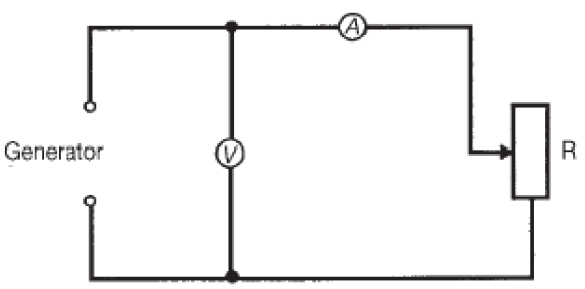
\includegraphics[width=0.6\linewidth]{att/schema.png}
				\caption{Schéma zapojení z \cite{bib:zadani}.}
				\label{fig:s_aparatura_moment}
					    	
				
		\end{center}
	\end{figure}
	

%\clearpage
\subsection{Grafy}

	\begin{figure}[h!]
	\begin{center}
	    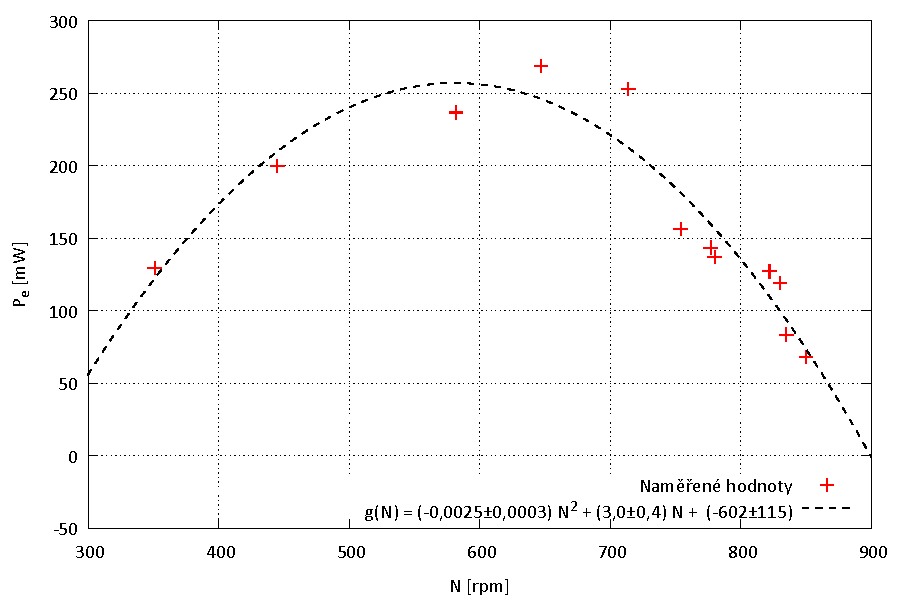
\includegraphics[width=\linewidth]{../gnuplot/12_stir.pdf}
	    	\caption{Graf elektrického výkonu $P_e$ v závislosti na frekvenci otáček motoru $N$. Naměřené hodnoty jsme proložili polynomem druhého stupně.}
			\label{fig:g_graf}
	\end{center}
	\end{figure}

\clearpage
    \begin{figure}[h!]
	\begin{center}
	    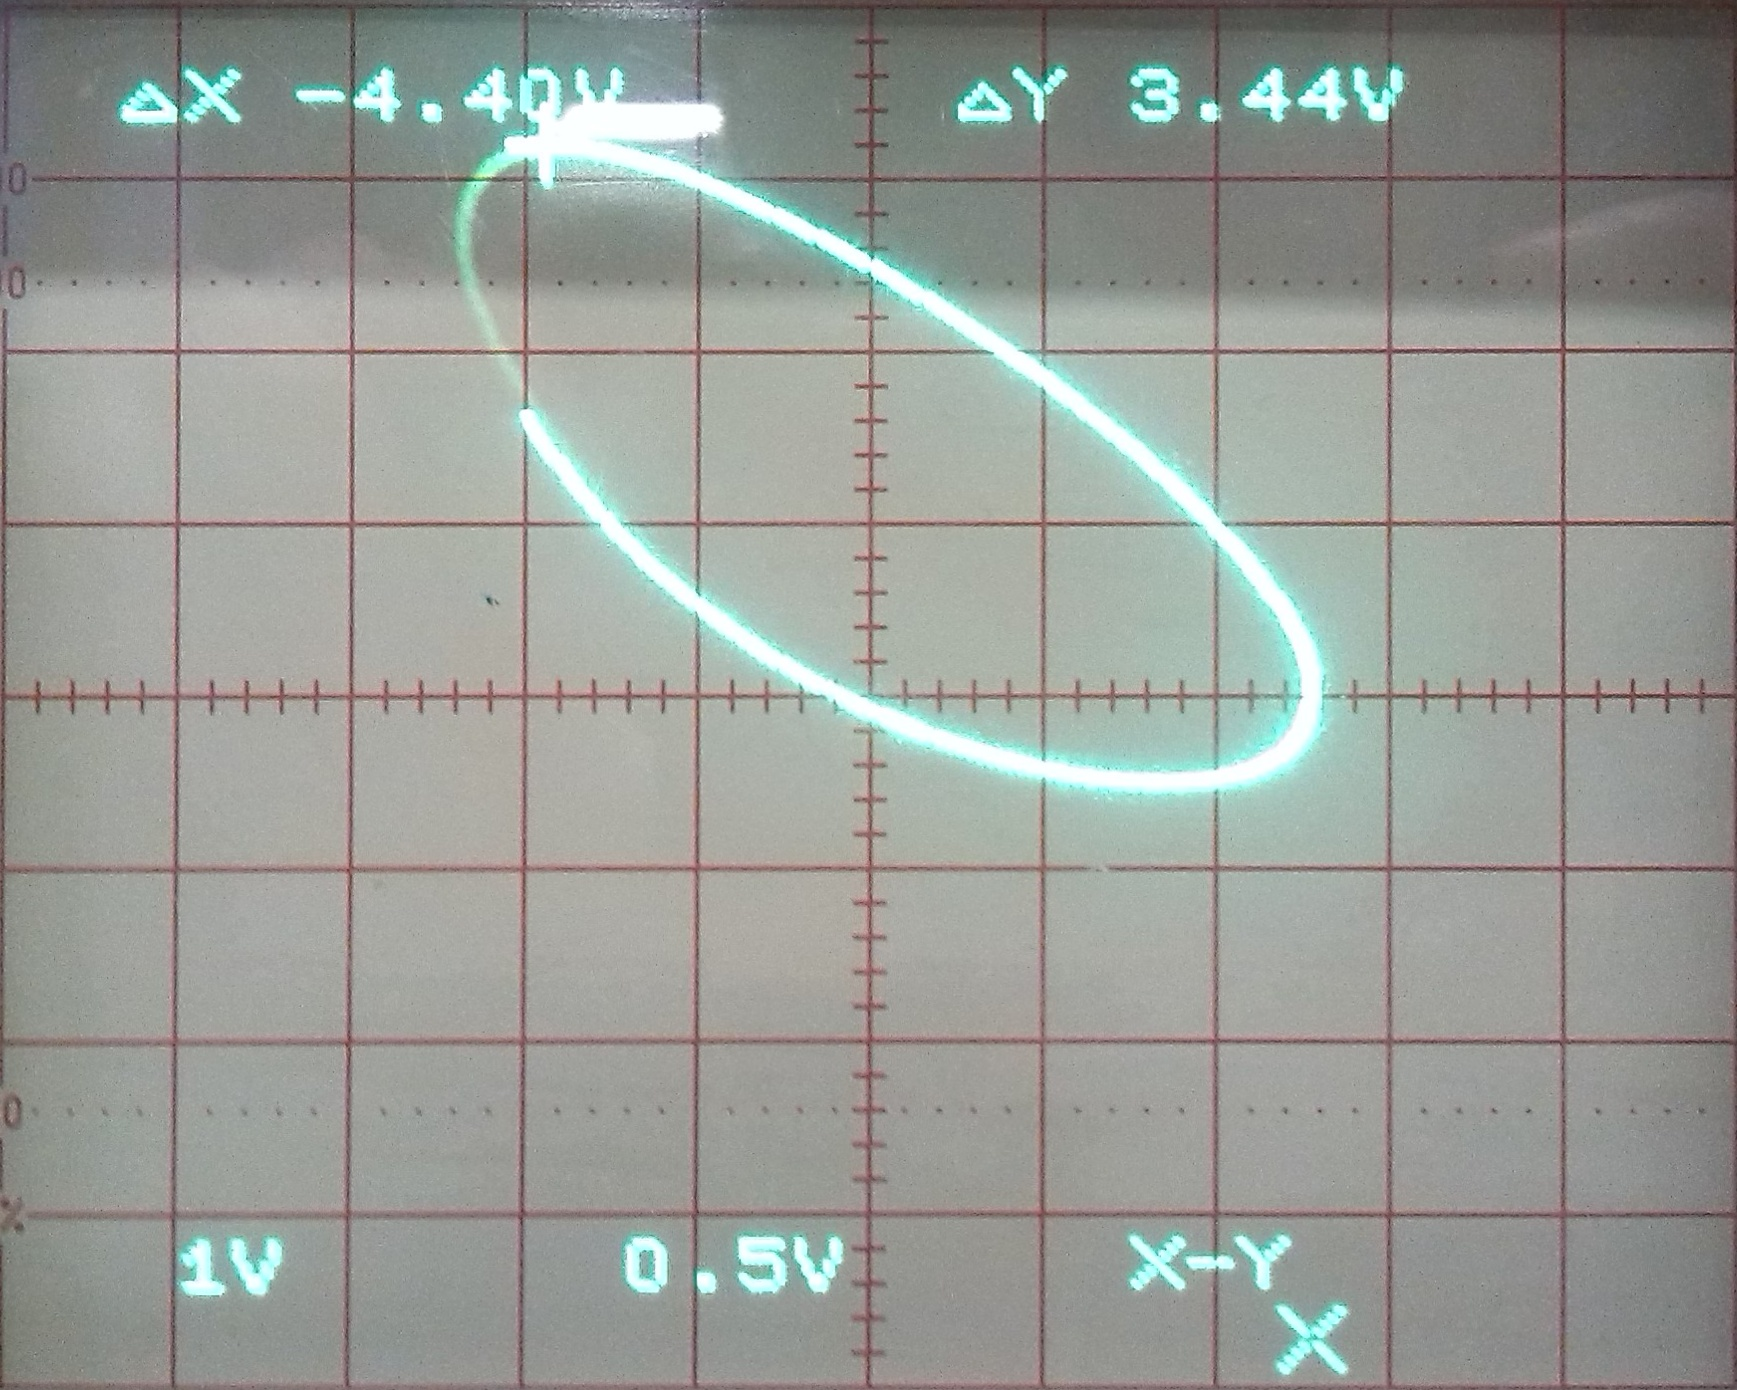
\includegraphics[width=10cm]{att/2.jpg}
	    	\caption{Záznam displeje z osciloskopu pro $N=835$ rpm.}
			\label{fig:o2}
	\end{center}
	\end{figure}
	
    \begin{figure}[h!]
	\begin{center}
	    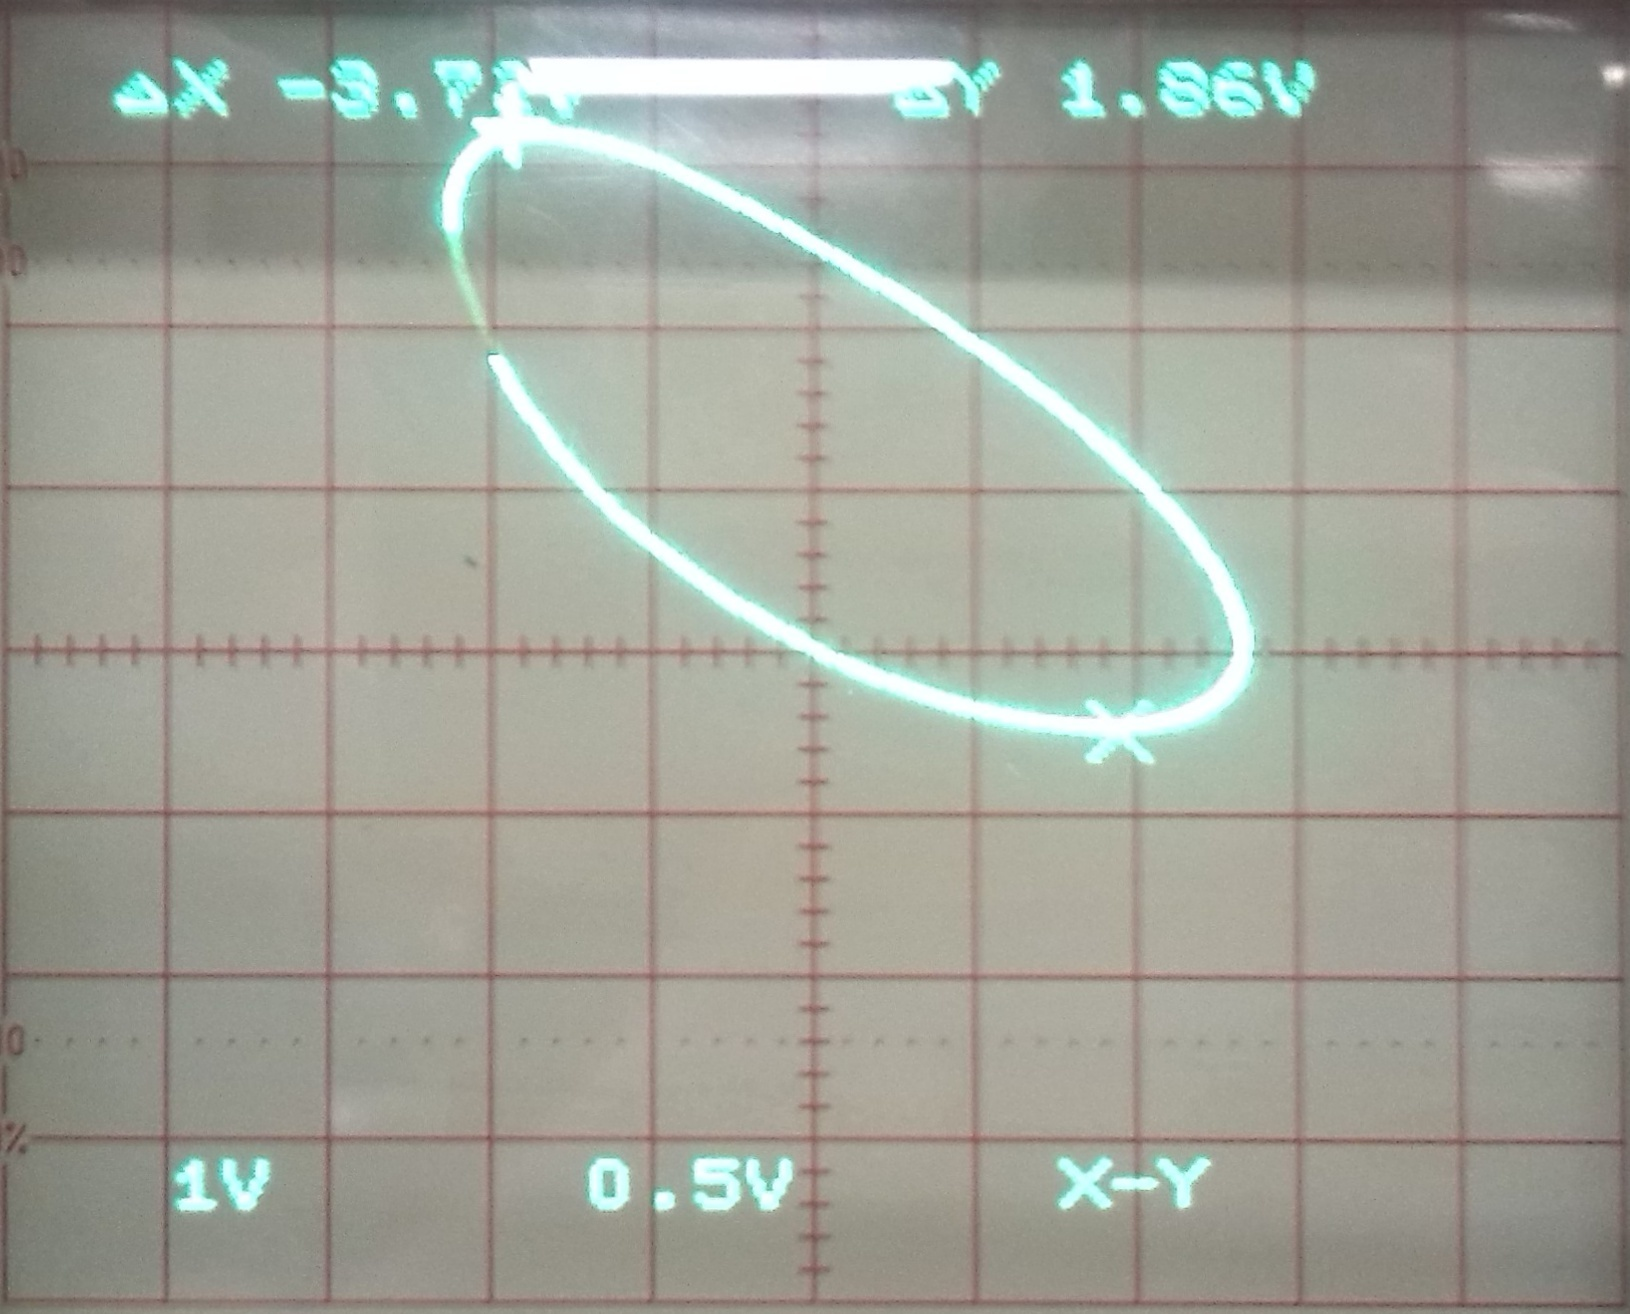
\includegraphics[width=10cm]{att/3.jpg}
	    	\caption{Záznam displeje z osciloskopu pro $N=830$ rpm.}
			\label{fig:o3}
	\end{center}
	\end{figure}

\clearpage

    \begin{figure}[h!]
	\begin{center}
	    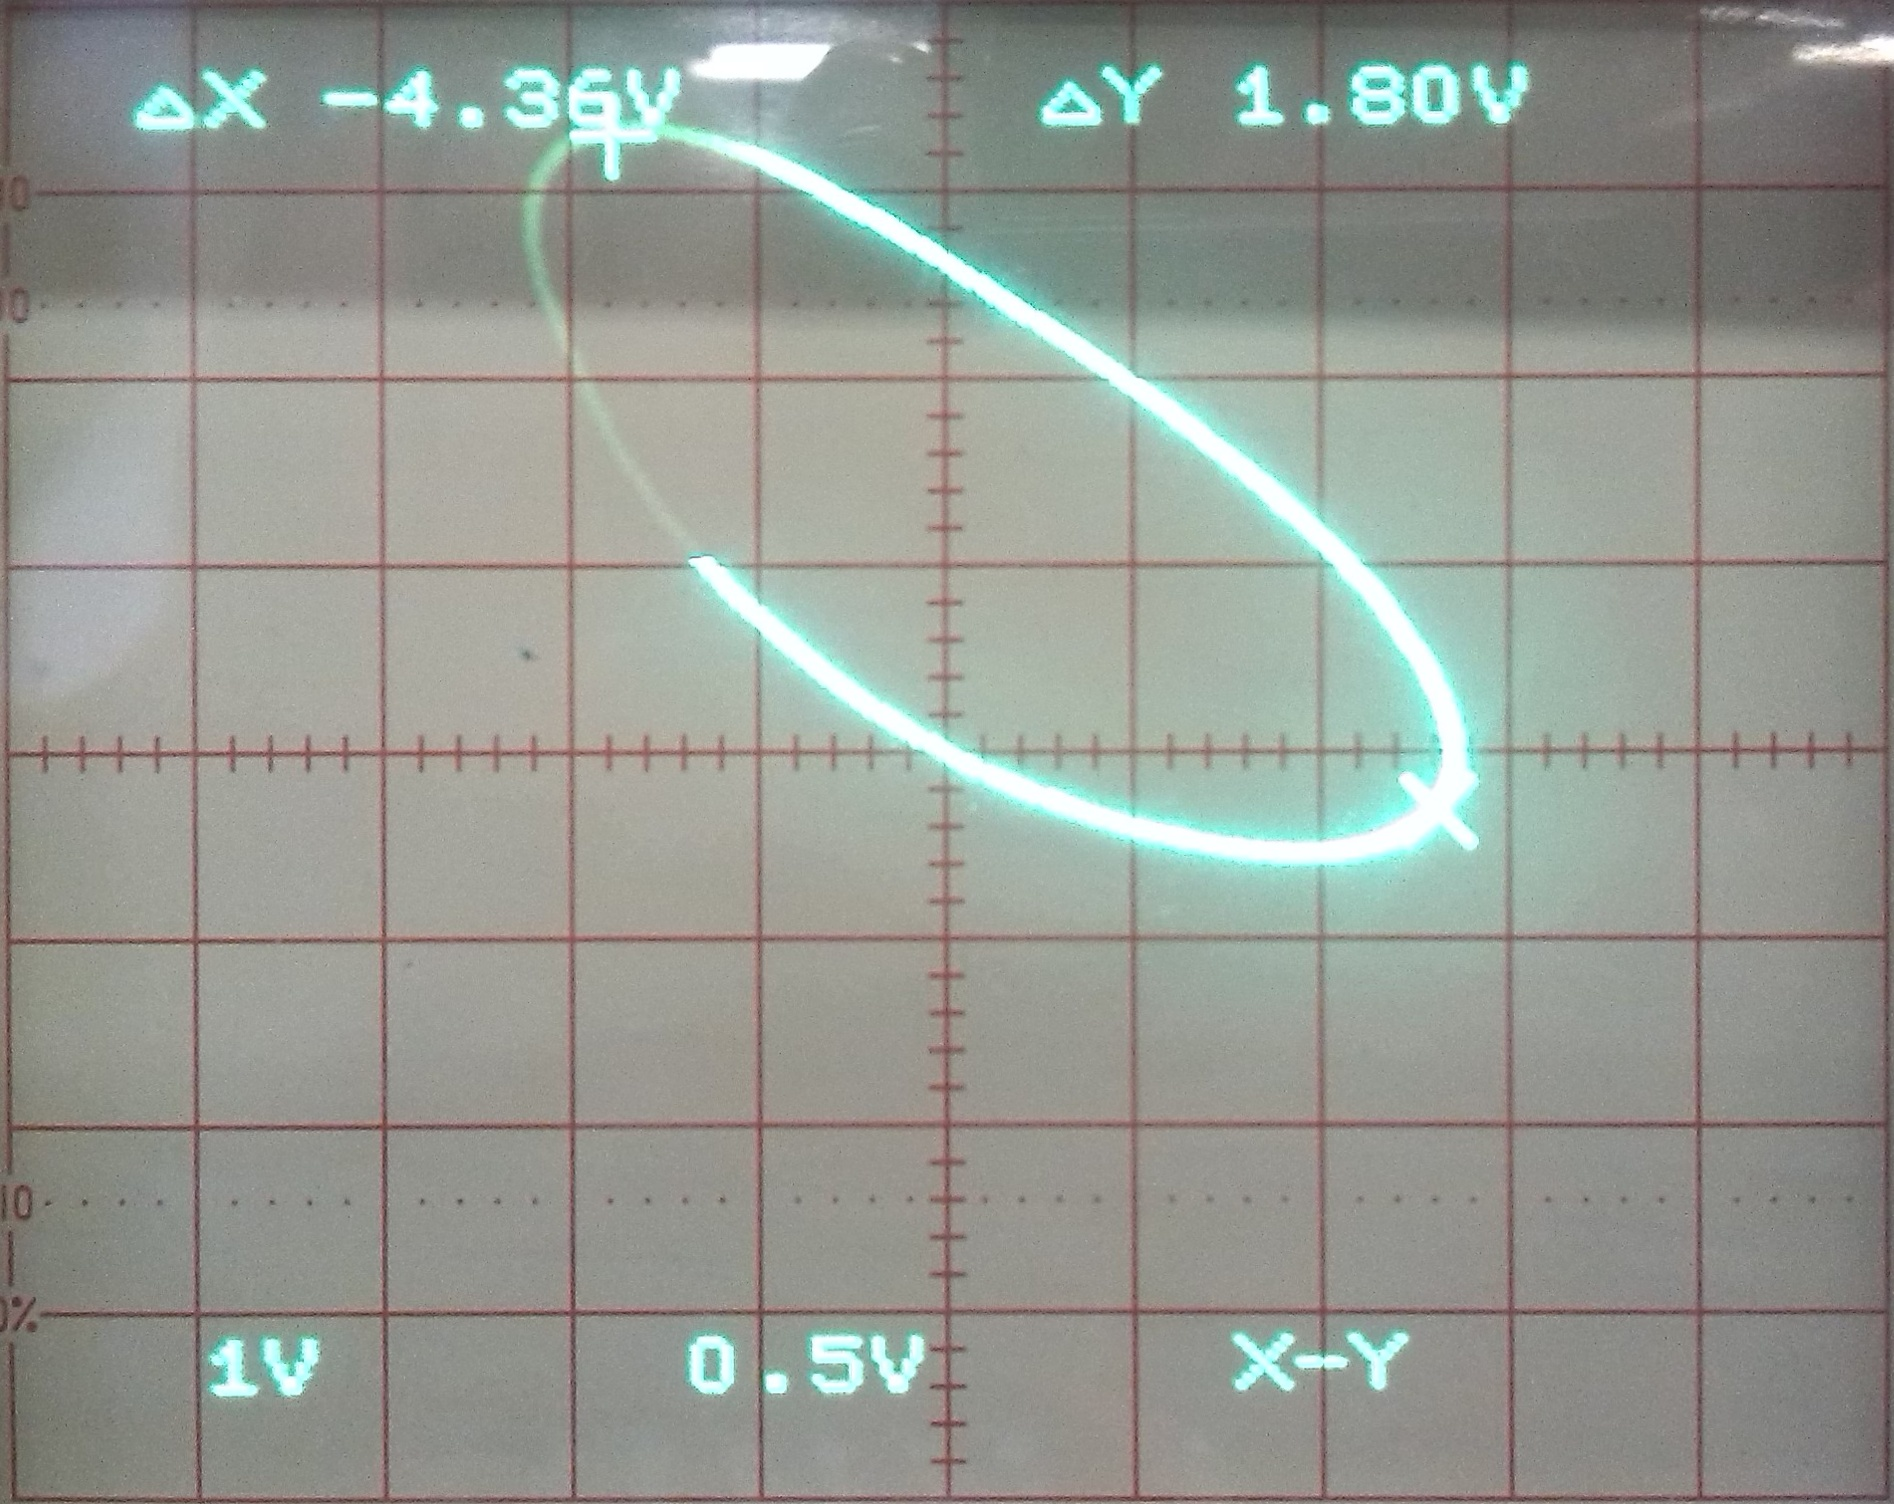
\includegraphics[width=10cm]{att/5.jpg}
	    	\caption{Záznam displeje z osciloskopu pro $N=647$ rpm.}
			\label{fig:o5}
	\end{center}
	\end{figure}

    \begin{figure}[h!]
	\begin{center}
	    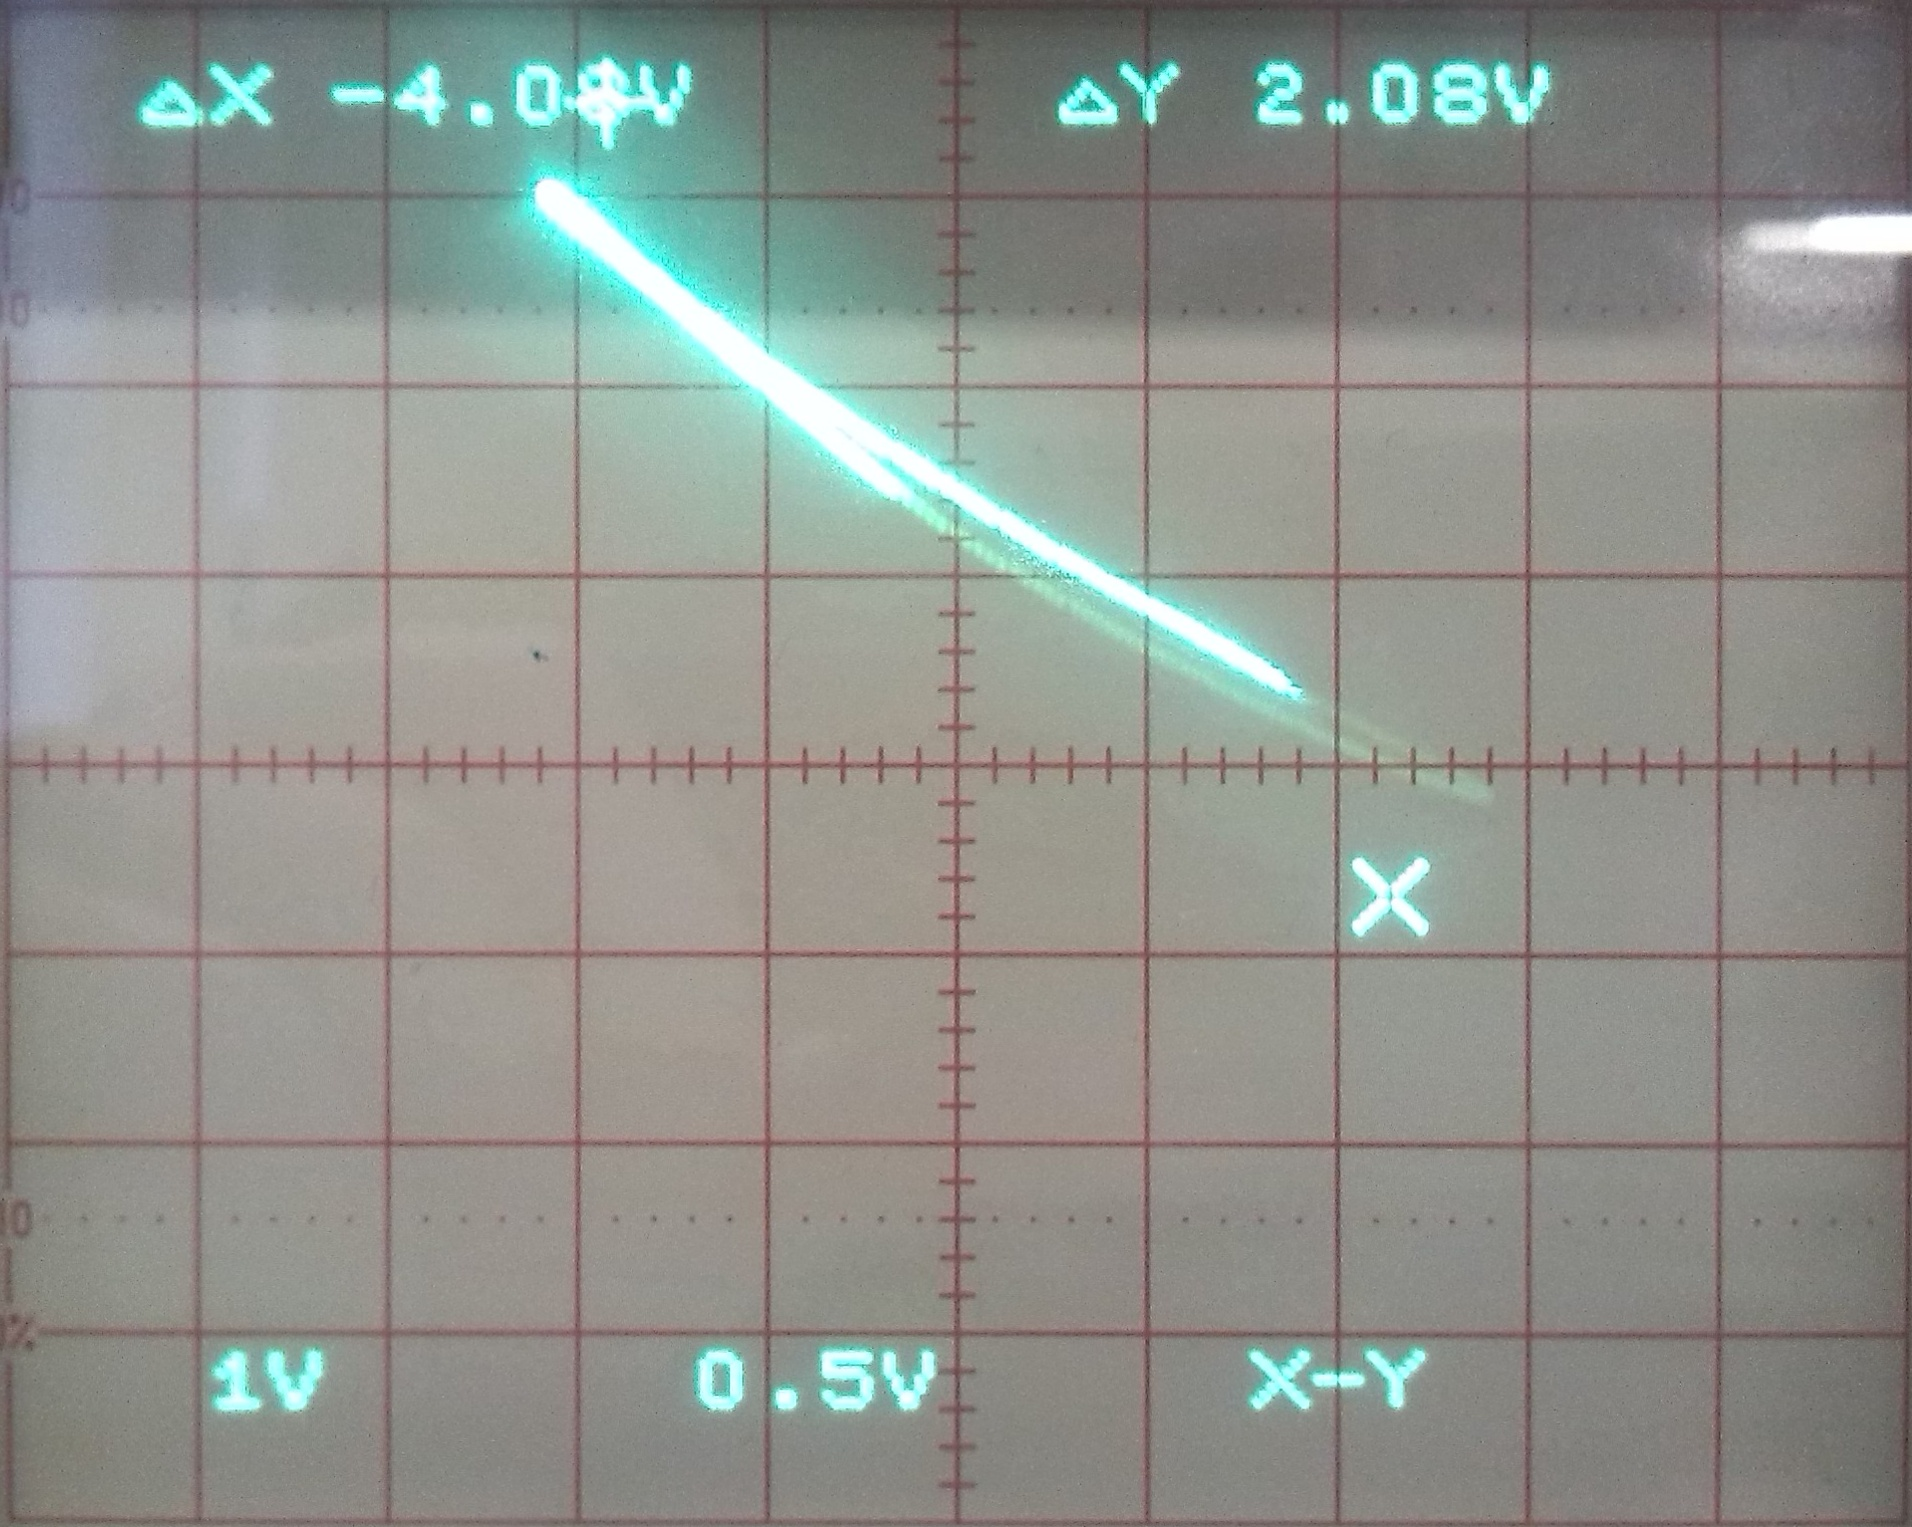
\includegraphics[width=10cm]{att/6.jpg}
	    	\caption{Záznam displeje z osciloskopu pro zapojení stroje jako chladničky.}
			\label{fig:o6}
	\end{center}
	\end{figure}	
	
% --- Konec dokumentu --------------------------------------------------


\end{document}

